\section{Sensitivity to $\alpha_s$}
\label{sec:sensitivity}

\cref{fig:alpha_results} shows aditional experiments on the sensitivity of our method to~$\alpha_s$ in the considered datasets.

%\begin{figure}[h]
%\centering
%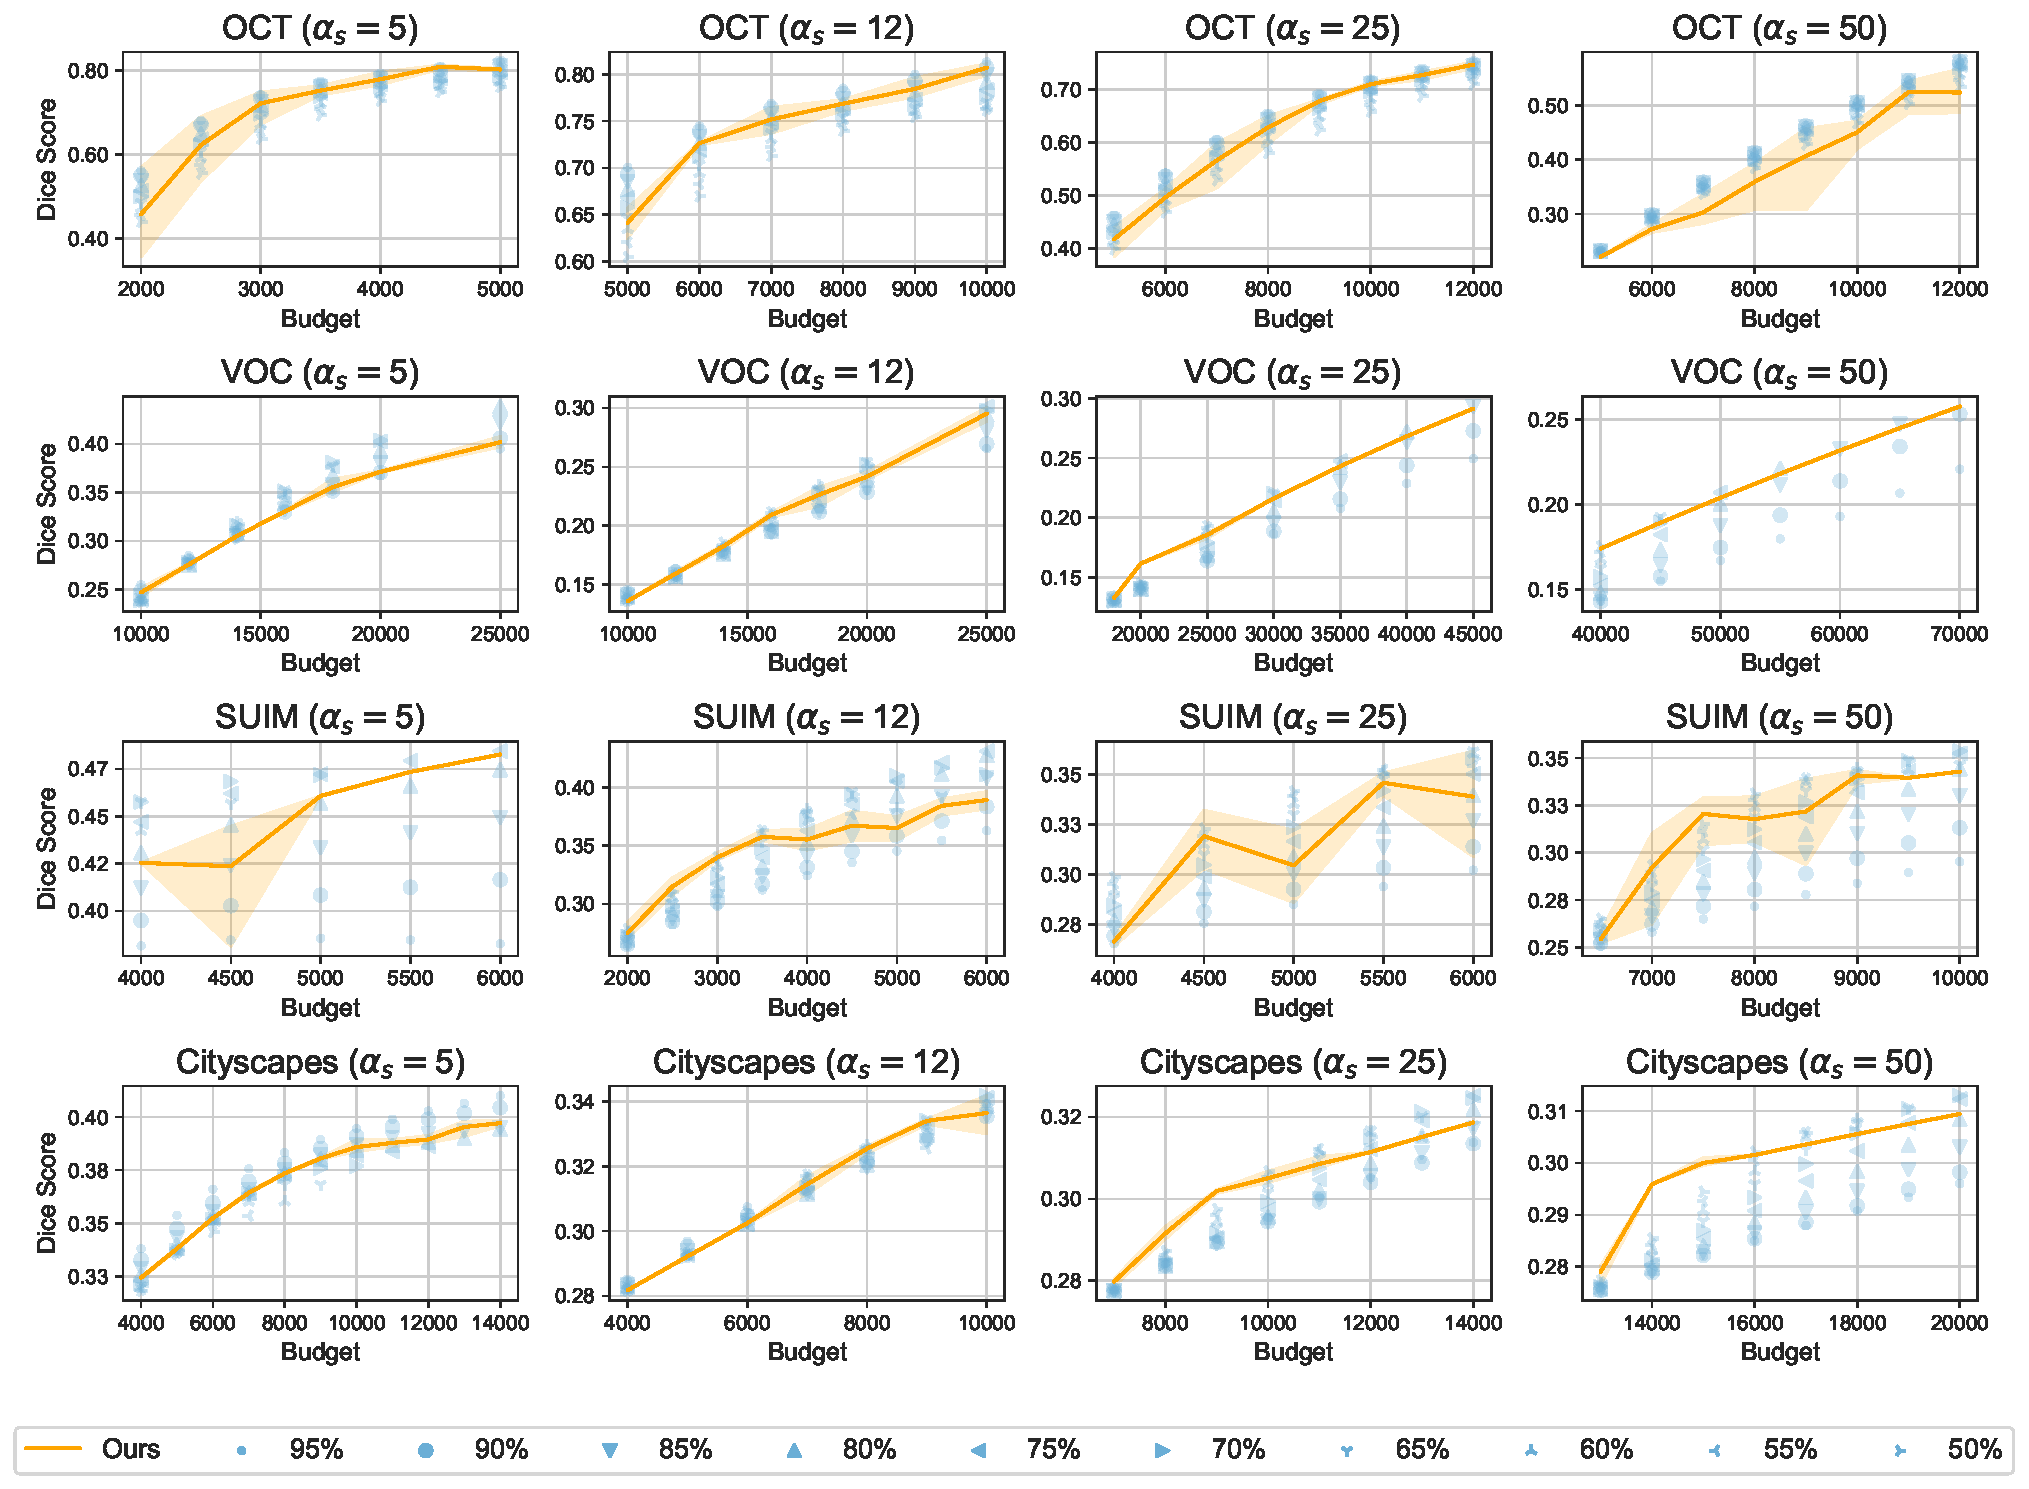
\includegraphics[width=\linewidth]{fullweak/Figures/alphas_notshared.pdf}
%\caption{Performance our method with $\alpha_s = \{5, 12, 25, 50\}$ on four datasets. One-sigma error bars were computed from three seeds. Blue marks show the performance of fixed strategies, with labels indicating the percentage of the budget allocated to segmentation annotations.
%}
%\label{fig:alpha_results}
%\end{figure}

\plainwidefig{1}{fullweak/Figures/alphas_notshared.pdf}{Performance our method with $\alpha_s = \{5, 12, 25, 50\}$ on four datasets. One-sigma error bars were computed from three seeds. Blue marks show the performance of fixed strategies, with labels indicating the percentage of the budget allocated to segmentation annotations.}{fig:alpha_results}